\documentclass[10pt,oneside,a4paper,final,english]{memoir}

\usepackage{palatino}
\usepackage{microtype}
\usepackage{lscape}
\usepackage{multicol}
%\usepackage{epic,eepic}
\usepackage{latexsym}
\usepackage{verbatim}
\usepackage{listings}
\usepackage{ulem}
\usepackage{hyperref}

\let\footruleskip\undefined
\usepackage{fancyhdr}
\usepackage[final]{fixme}

\let\fref\undefined
\usepackage[plain]{fancyref}

%% FOR LOOP
\usepackage{ifthen,calc}
\newcounter{myforloopcounter}
\newcommand{\forloop}[5][1]% 
{\setcounter{#2}{#3}% 
\ifthenelse{#4}% 
{#5%
  \addtocounter{#2}{#1}% 
  \forloop[#1]{#2}{\value{#2}}{#4}{#5}% 
}%
% Else 
{}%
}% 


%% USAGE
%\forloop[step]{counter}{initial_value}{conditional}{code_block} 
\usepackage[english]{babel}
\usepackage[utf8]{inputenc}

%\selectlanguage{danish}

\lstset{language=Python,basicstyle=\small,
  columns=fullflexible}


\usepackage[pdftex]{graphicx}

\DeclareGraphicsExtensions{.jpg .png .pdf}


\usepackage{amsmath}
\usepackage{latexsym}
\usepackage{amssymb}


\usepackage[osf,sc]{mathpazo}
\usepackage{microtype}
%\usepackage{fourier}
\linespread{1.05}

%\usepackage[charter]{mathdesign}
%\usepackage{lmodern}

%\usepackage{algorithmic}
%\usepackage{algorithm}

\usepackage{amsthm}


\theoremstyle{plain}  \newtheorem{definition}{Definition}
\theoremstyle{remark} \newtheorem{lemma}{Lemma}
\theoremstyle{plain}  \newtheorem{theorem}{Theorem}
\theoremstyle{remark}  \newtheorem{example}{Example}


\newcommand{\p}{\ensuremath{^\prime}}
\DeclareGraphicsExtensions{.jpg, .eps, .png}
%%% Local Variables:
%%% mode: plain-tex
%%% TeX-master: "../master"
%%% End:

\usepackage{algorithmic}
\usepackage{algorithm}
\usepackage[sectionbib,square]{natbib}
%\bibpunct{(}{)}{,}{a}{}{}
\setcitestyle{alpha}
%\setcitestyle{numbers,aysep={},yysep={;}}

\usepackage{datetime}

\chapterstyle{thatcher}

%\pagestyle{fancy}
\begin{document}
  \fontencoding{T1}
%  \fontseries{m}
%  \fontshape{n}
%  \fontsize{12}{15}
%  \selectfont


%%%%%%%%%%%%%%%%%%%%%%%%%%%%%%%%%%%%%%%%%%%%%%%%%%%%%%%%
%                    Forside
%%%%%%%%%%%%%%%%%%%%%%%%%%%%%%%%%%%%%%%%%%%%%%%%%%%%%%%%
\makeatletter % open mode for reading @ signed variables
\def\maketitle{%
 \null
 \thispagestyle{empty}%
 \vfill
 \begin{center}\leavevmode
   \normalfont
   \LARGE{\raggedleft \@title\par}%
   \hrulefill\par
   \large{\raggedleft \subtitle\par}%
   \vskip 2cm
   {\today\par}%
 \end{center}%
 \vfill
 \begin{flushleft}
   {\large \@author } \\
   {\footnotesize \suplementInfo }
 \end{flushleft}
 \clearpage % Terminates the page here. Everything else vil be placed
            % on next page.
}
\makeatother % closing mode for reading @ signed variables
%%%%%%%%%%%%%%%%%%%%%%%%%%%%%%%%%%%%%%%%%%%%%%%%%%%%%%%%
%               Data til forside
%%%%%%%%%%%%%%%%%%%%%%%%%%%%%%%%%%%%%%%%%%%%%%%%%%%%%%%%
\title{Final Hand In $\cdot$ Week VIII}

\def\subtitle{CCO $\cdot$ Constraint Continuous Optimization}

\author{Johan Sejr Brinch Nielsen} \def\suplementInfo{

\kern 5pt \hrule width 11pc \kern 5pt

\begin{tabular}{ll}
Email: & zerrez@diku.dk  \\
Cpr.:  & 260886-2547
\end{tabular}

% putter 5pt spacing oven over og neden under stregen
\kern 5pt \hrule width 11pc \kern 5pt

Dept. of Computer Science,  \\
University of Copenhagen

}


\maketitle
\newpage


\section{Introduction}
The assignment is the describe and implement the Levenberg-Marquardt
algorithm and compare this to last weeks Newton's method. Interesting
comparisons could be based on number of iterations used, the precision
of the solution found and the algorithms robustness.



\section*{A: Levenberg-Marquardt Algorithm}

The Levenberg-Marquardt algorithm has a lot of similarities with
Newton's method. Both are iterative root-finding algorithms and both
compute a new direction in each step. However, where Newton's method
computes the new direction using a simple Taylor approximation,
Levenberg-Marquardt uses a combination of approximation and deepest
descent. Intuitively, the algorithm uses long steps as long as this
approach results in improved values. When a long step does no longer
work, the algorithm gradually reduces the step size.

The Levenberg-Marquardt update value is defined as:
\[ \Delta = - (J^TJ - \lambda I)^{-1} J^T r\]

Where $J$ is the jacobian matrix, $\lambda$ is the step modifier,
$r$ is the residual vector and $\Delta$ is the next modification of
the approximation.
When the step modifier $\lambda$ gets large, it will dominate the
inverted matrix, such that:
\[ \Delta \approx - (-\lambda I)^{-1} J^T r = \]
\[ - \frac{1}{\lambda}I J^T r \]

It is now clear why $\lambda$ is a step modifier. A large $\lambda$
implies a small $\Delta$. Also, $\lambda$ determines whether $J^TJ$ or
$-\lambda I$ should dominate the direction. In the latter case, the
direction is determined by $J^T$, that is the first order partial
derivatives. This is the same direction as the steepest descent method
would have chosen and it is this trick, that is the key to the
convergence of Levenberg-Marquardt. Since the $\lambda$ value is
multiplied by a positive factor when no better approximation is
available, the method will eventually find a better point closer to
the goal.



\section*{B: Comparison to Week1 Implementation}
\subsubsection*{Explanation of Pictures}
Each picture contains four plots. Here described from left to right,
row by row.
\begin{enumerate}
\item The plot in the upper left corner shows the solution chosen by
  Newton's method.
\item The plot in the upper right corner shows the solution chosen by
  the Levenberg-Marquardt method.
\item The plot in the lower left corner shows the logarithmic error,
  for each iteration, for Newton's method.
\item The plot in the lower right corner shows the logarithmic error
  for each iteration, for Levenberg-Marquardt.
\end{enumerate}

\begin{center}
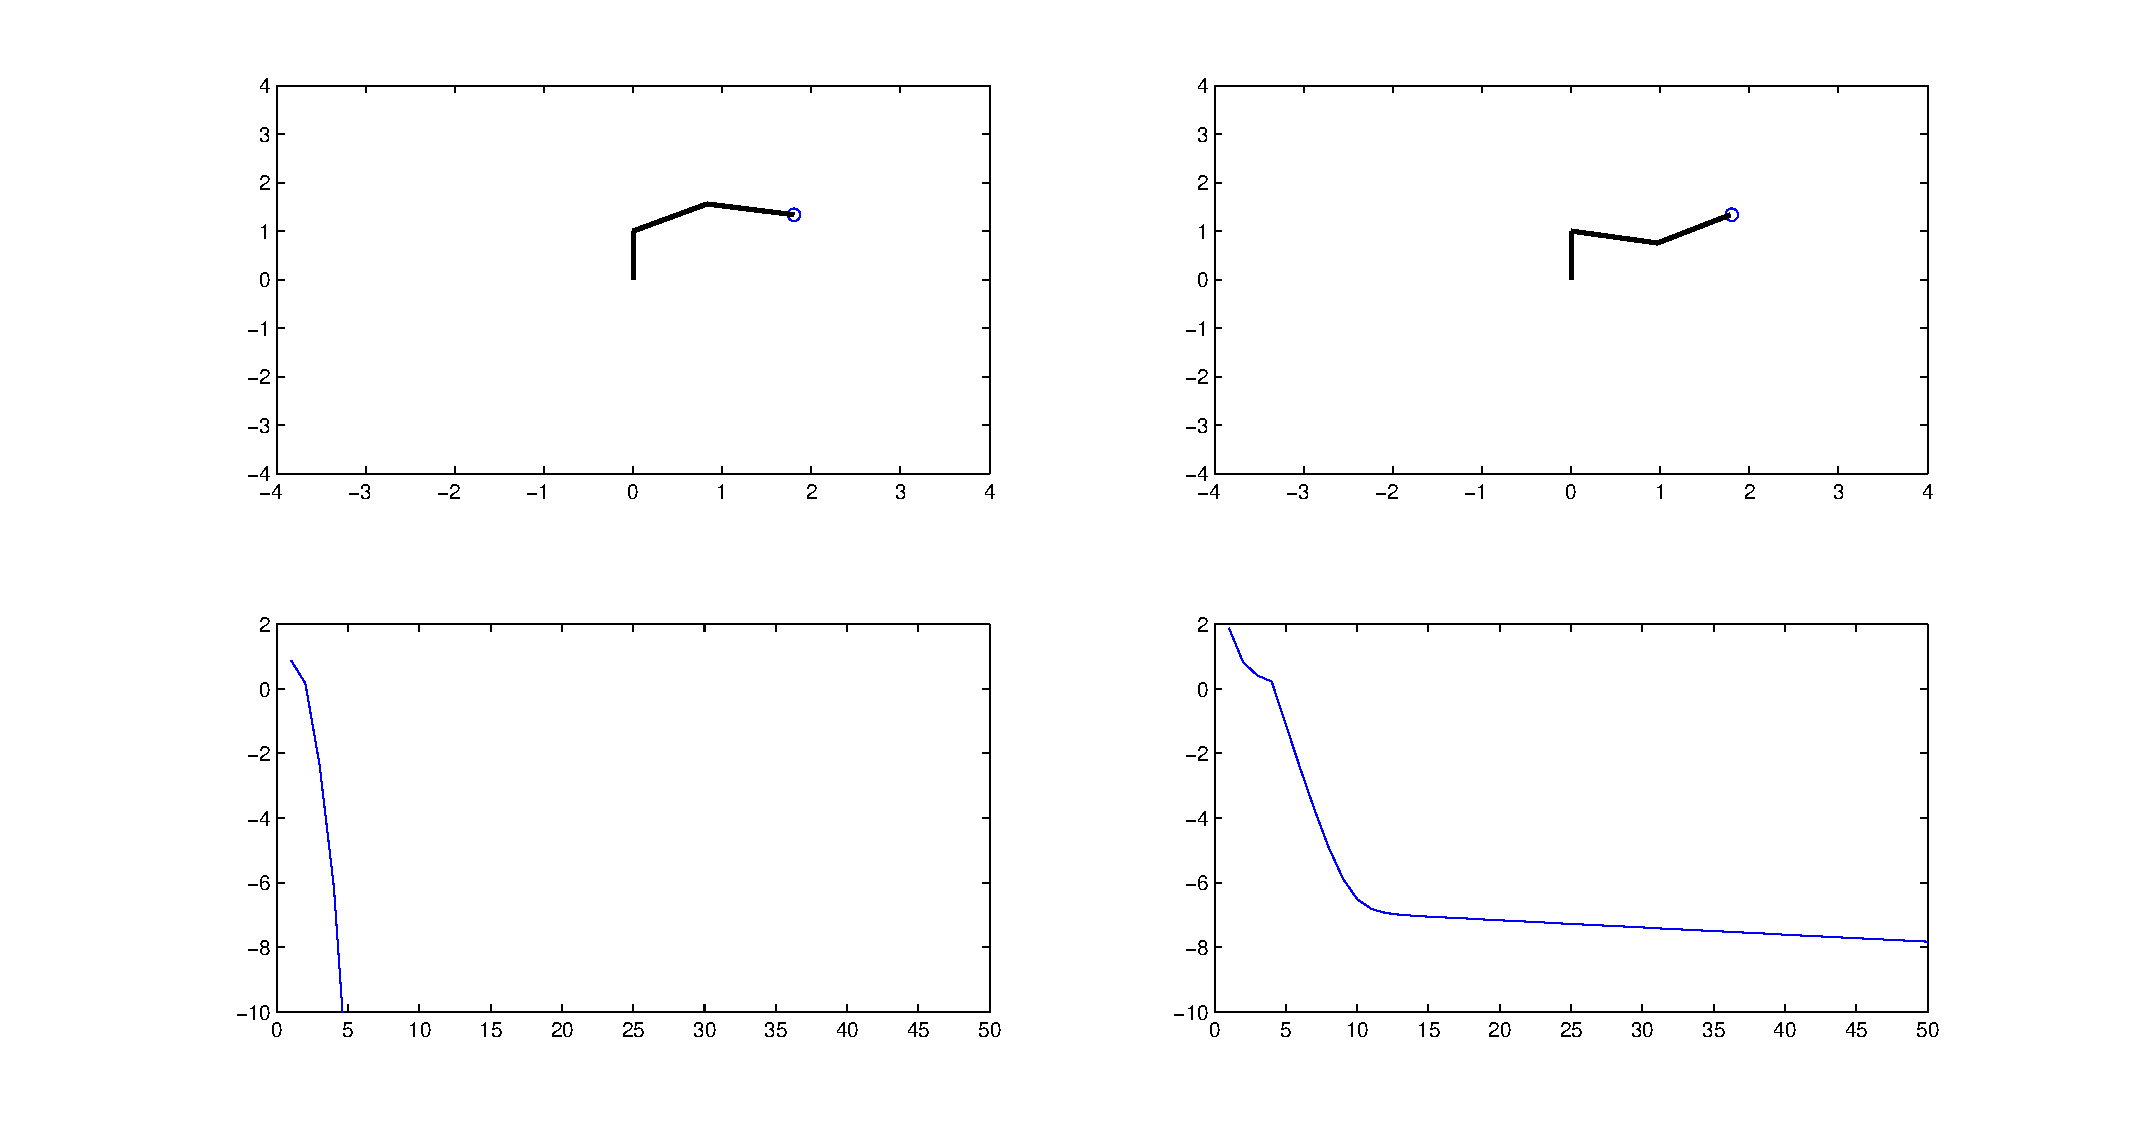
\includegraphics[width=\textwidth]{images/shot1.pdf}\\
\end{center}
This graph shows the two algorithm's solutions to the same goal. Both
algorithms finds a solution that seems close to the wanted point,
however the error graphs clearly show that Newton's method is both
faster and more precise. In fact, Newton's method is very fast in this
case. Notice how Levenberg-Marquardt converges quadratically at first
and then turn linear when steepest descent kicks in.



\begin{center}
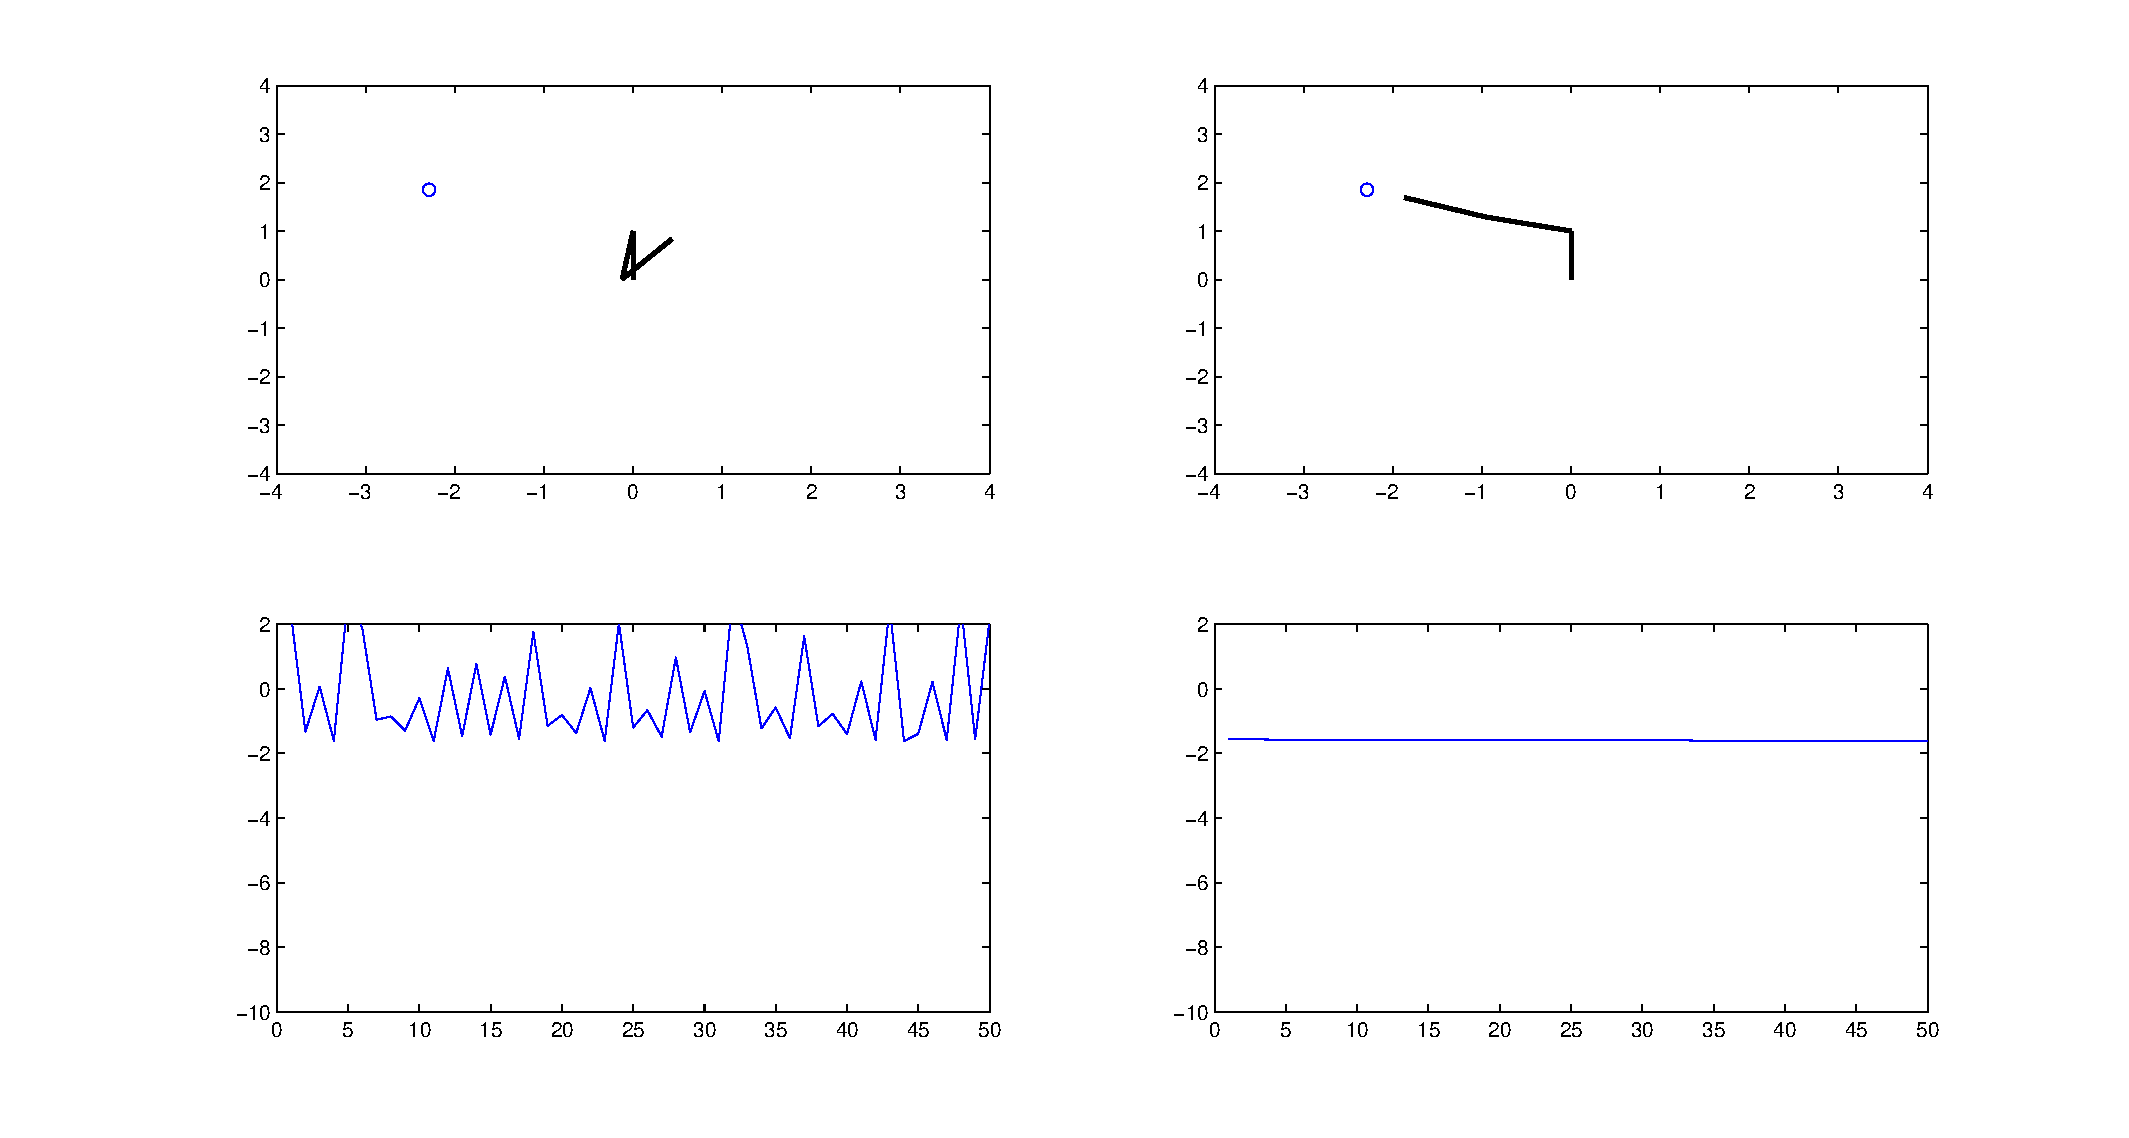
\includegraphics[width=1\textwidth]{images/shot2.pdf}\\
\end{center}
This is a case where the goal point lies outside the reach of the
arm. It is not possible to actually reach it. It is here the steepest
descent trick of Levenberg-Marquardt comes into play. While this
ensures a solution in the right direction, Newton's method fails to
find one. This suggests that Levenberg-Marquardt is more robust. Note
however, that steepest descent is quite slow.


\begin{center}
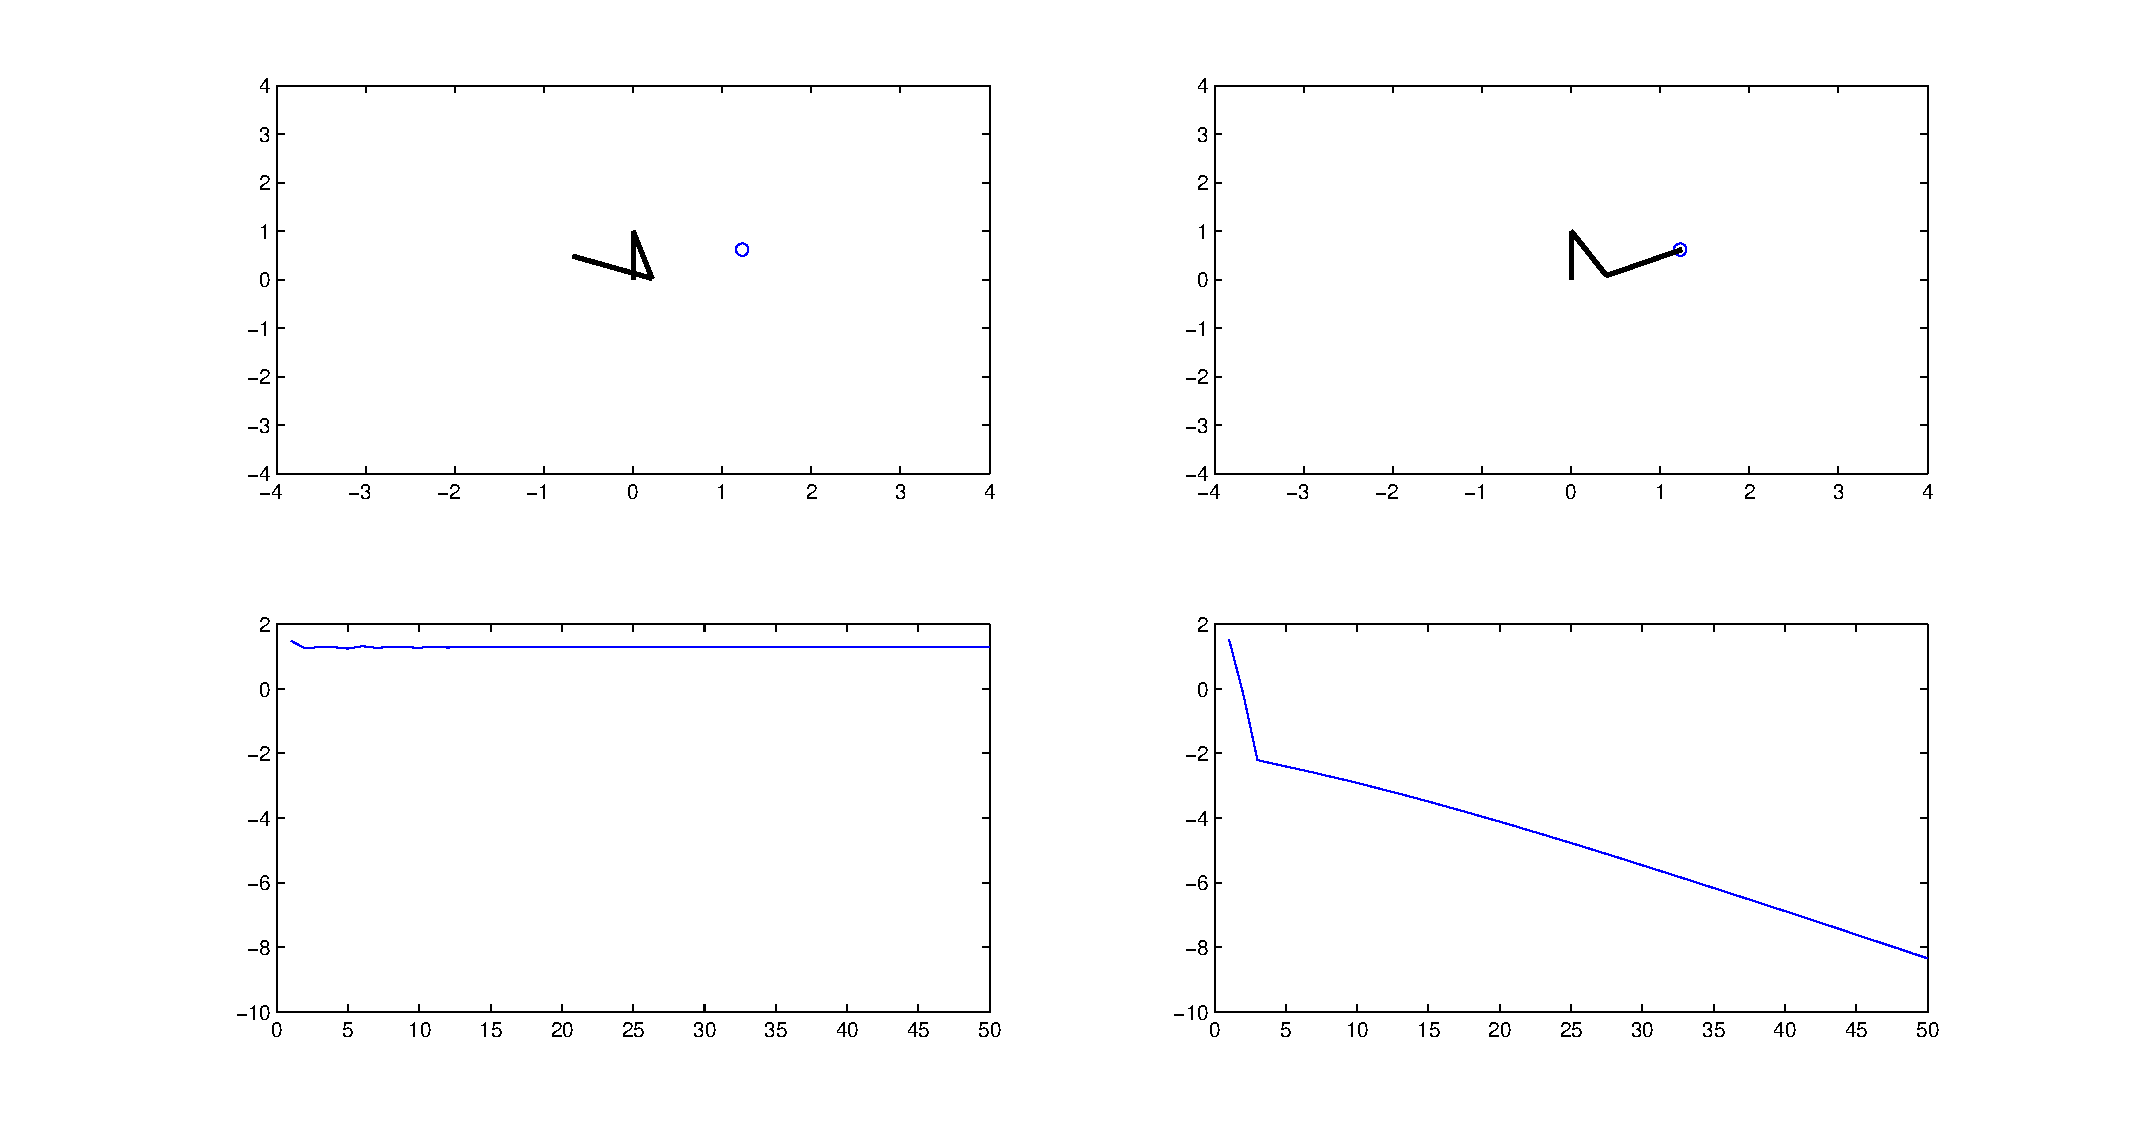
\includegraphics[width=1\textwidth]{images/shot3.pdf}\\
\end{center}
This is an interesting plot. The point chosen lies within reach of the
arm, but the initial guess is far from it (all to the left). This
fools Newton's method, that doesn't seem to get anyway in the 50
iterations. Levenberg-Marquardt finds the solution with something
that looks like a linear convergence rate. The bend it its curve
suggest is most likely a flip to steepest descent.



\section*{Implementation}
This section contains the modified pseudo code and MatLab code for
this week's programming case.
\subsection*{Pseudo Code for LM}

This is my pseudo code for the Levenberg-Marquardt algorithm. In the
implementation, the inner for-loop has been replaced by a while-loop.
\begin{verbatim}
def LevenbergMarquardt(f, goal):
  ld = 0.0001, c = 2, x = 0
  endPoint = f(x)
  oldError = || goal - endPoint ||
  for i = 1 to N:
    dt = LMupdate(ld, goal - endPoint)
    newEndPoint = f(x + dt)
    newError = || goal - newEndPoint ||
    if newError >= oldError
      ld = ld * c
      REJECT
    else
      ld = ld / c
      oldError = newError
      x = x + dt
      ACCEPT
    fi
  rof
fed
\end{verbatim}


\subsection{MatLab Code}
\paragraph{LMupdate}

This is my MatLab code for the helper function \texttt{LMUpdate}:
\begin{verbatim}
function [ delta ] = LMupdate(lambda, J, r)
  tJ = transpose(J);
  delta = -inv(tJ*J - lambda * eye(size(J))) * tJ * r;
end
\end{verbatim}


\paragraph{Levenberg-Marquardt}

This is my MatLab code for the Levenberg-Marquardt algorithm:
\begin{verbatim}
function [ angles ] = levenberg_marquardt( goal, t, angles )
%
% input
%     g      : Goal position/vector (specified in homogenuous coordinates)
%     t      : A vector of fixed rod-link vectors
%     angles : A vector with joint angles
%     e      : Position/vector (specified in homogenuous coordinates)
% output
%     angles : The updated pose which will reach the specified goal position.

e  = [0;0;1];
endPoint = f(t, angles);

iter = zeros(1,50);
err  = zeros(1,50);

lambda   = 0.0001;

oldError = dot(goal-endPoint,goal-endPoint);

for i = 1:50
    % Compute new angles, endpoint and error
    r = goal - endPoint;
    J = jacobian(t, angles, e);

    % Keep doubling lambda until error is reduced
    newError = oldError + 1;
    while newError >= oldError
        % REJECT
        lambda = lambda * 2;
        delta = LMupdate(lambda, J, r);
        newAngles   = angles + delta;
        newEndPoint = f(t, newAngles);
        error = goal-newEndPoint;
        newError = dot(error, error);
    end

    % ACCEPT
    oldError = newError;
    angles   = newAngles;
    endPoint = newEndPoint;
    lambda = lambda / 2;

    % Remember observed error
    err(i)  = log(oldError);
    iter(i) = i;
end

subplot(2,2,4);
plot(iter, err);
axis([0 50 -10 2]);
subplot(2,2,1);

end
\end{verbatim}


\paragraph{Run}

I also changed the code in the file ``run.m'' to get support more
advanced figures with 4 plots on each:
\begin{verbatim}
% Make sure we got a clean environment to work in
close all;
clear all;

% Setup a default configuration
t      = [ 0 0 0; 1 1 1];
angles = [pi/4; pi/4; pi/4];

% Try to find end-effector position
e = f(t, angles);

% Get x and y coordinates
x = e(1);
y = e(2);

% Verify if f worked as we expected
if ( (x  + 1.7071) > 0.001 )
    error('x-test failed.');
end

if (  (y  - 1.7071) > 0.001 )
    error('y-test failed.');
end

figure(1);

clf;
hold on;
title('Inverse Kinematic Chain');
xlabel('X');
ylabel('Y');

subplot(2,2,1);
draw_chain( t, angles );
subplot(2,2,2);
draw_chain( t, angles );

theaxis = [-4 4 -4 4];
angles = ones(size(angles));
for n = 1:20
    % Newton
    subplot(2,2,1);

    [gx,gy] = ginput(1);
    plot(gx,gy,'bo');

    new_angles = nonlinear_newton([gx; gy; 1],t,angles);
    subplot(2,2,1);
    draw_chain( t, new_angles );

    axis(theaxis);

    % Levenberg
    subplot(2,2,2);
    plot(gx,gy,'bo');
    angles = levenberg_marquardt([gx; gy; 1],t,angles);
    subplot(2,2,2);
    draw_chain( t, angles );

    axis(theaxis);
end
hold off;
\end{verbatim}

\paragraph{newton\_gauss}

And lastly, I updated my Newton's method code from last week to draw
error plots:
\begin{verbatim}
function [ angles ] = nonlinear_newton( g, t, angles )
%
% input
%     g      : Goal position/vector (specified in homogenuous coordinates)
%     t      : A vector of fixed rod-link vectors
%     angles : A vector with joint angles
%     e      : Position/vector (specified in homogenuous coordinates)
% output
%     angles : The updated pose which will reach the specified goal position.

e  = [0;0;1];
ep = f(t, angles);

iter = zeros(1,50);
err  = zeros(1,50);
for i=1:50
    da = pinv(jacobian(t, angles, e))*(g - ep);
    angles = angles + da;
    ep = f(t, angles);
    error = g-ep;
    err(i)  = log(dot(error,error));
    iter(i) = i;
end

subplot(2,2,3);
plot(iter, err);
axis([0 50 -10 2]);

end
\end{verbatim}




\end{document}

%%% Local Variables:
%%% mode: latex
%%% TeX-master: t
%%% End:
